\section{PixelCNN}

\subsection{Overview}

Introducing the VQ-VAE, we have seen that an under-table tool that was being used is the Pixel CNN,
first introduced in \cite{pixel_cnn_paper}.
In the context of the VQ-VAE, it plays a major role after training by learning the prior $p(z)$, that was set
to a discrete uniform previously.
This makes a drastic difference with the VAE, as we are not setting the prior ourselves as it's being learnt and modeled by the PixelCNN in this process.
\medskip

Indeed, the PixelRNN/PixelCNN architectures are sequential deep neural networks that aims at modeling the distribution of a data space
in an autoregressive fashion.
Their main characteristic is that they take advantage of the structure of an image to learn the data space distribution.
\begin{itemize}
    \item \textit{PixelRNN}: Bi-directional recurrent networks with variable smart directions are used to model the spatial dependencies between pixels.
    (3 architectures are presented in the original paper, but our focus will be on the PixelCNN here).

    \item \textit{PixelCNN}: the dependencies between the pixels is modeled through stacking of masked convolution layers (it's faster since the receptive field is bounded by the size of the convolution), no pooling layer is used.
    The masking ensures that we keep an autoregressive estimation of a new pixel, without seeing the future pixels.
\end{itemize}

The following figure illustrates the masked convolution technique.
\begin{figure}[H]
    \center
    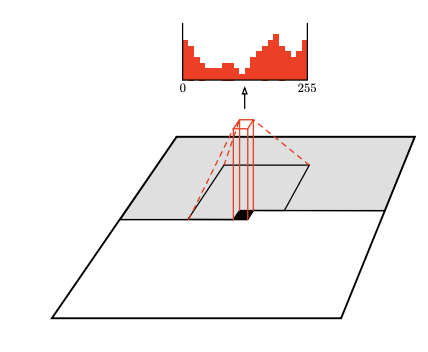
\includegraphics[scale=0.9]{images/masked_convolution_pixel_cnn}
    \caption{Masked convolution on an image (largest square), the big square represents the receptive field of the black pixel, the white area is masked}
    \label{fig:masked_convolution_pixel_cnn}
\end{figure}

Hence, given $x$ an image represented by its pixels $x = (x_1, \dots, x_n)$, as usual for these distribution modeling problems, we aim at finding $\theta^* = arg\max_{\theta} p_{\theta}(x)$ in a family of distributions parameterized by $\theta$: the maximum of likelihood.
Contrary to the usual independent framework, we consider a local dependency between pixels given by the receptive field of our convolution.
This local dependency is limited to the already seen pixels only as well, thanks to the masked convolution.
\medskip

Furthermore, rather than using continuous outputs, these architecture use a softmax layer to determine the pixel of a given generation,
leading to a discrete prior rather than a continuous one, which is required for the VQ-VAE for instance.
As a result, the distribution of a pixel conditionally to the ones in its receptive field is given by a multinomial in $\{0, \dots, 256\}$.
\medskip

\subsection{Usage in the VQ-VAE}

Once we have trained the VQ-VAE, the original paper states that we can replace the uniform prior on $p(z)$ by a PixelCNN to model the prior.
To perform the training of the PixelCNN, we turn the samples $x$ in their latent representations $z$, and train the PixelCNN over the latent representations $z$.
This way, we have created dependency between the $z$ in the latent feature mapping, and we obtain a prior over their distribution modeled by the PixelCNN.

